\chapter{Frequency-Shift Keying (FSK)}
\label{ch:fsk}

\begin{nontechnical}
\textbf{FSK is like Morse code with two different musical notes}---high note = 1, low note = 0. Simple, robust, and still used everywhere!

\textbf{Musical analogy:}
\begin{itemize}
\item Playing piano: \textbf{C note} = bit 0, \textbf{E note} = bit 1
\item Song: ``C C E C E E C'' = data: ``0 0 1 0 1 1 0''
\item Your ear (receiver) easily distinguishes C from E!
\item FSK receiver does the same with radio frequencies
\end{itemize}

\textbf{Why it's great:} Noise changes amplitude, but frequency stays clear! Immune to fading---signal can get weaker, but frequency doesn't change.

\textbf{Where you hear it:}
\begin{itemize}
\item \textbf{Caller ID}: Your phone uses FSK between rings
\item \textbf{Fax machines}: Those alternating tones you can hear
\item \textbf{Dial-up modems}: BEEEE-doo-BEEEE-doo (remember the 90s?)
\end{itemize}

\textbf{Modern uses:} Bluetooth Low Energy (GFSK), LoRa IoT networks, weather balloons, RFID tags.
\end{nontechnical}

\section{Overview}

\textbf{Frequency-Shift Keying (FSK)} is a digital modulation scheme where binary data is represented by switching between two discrete carrier frequencies.

\begin{keyconcept}
FSK provides \textbf{excellent immunity to amplitude variations} and \textbf{non-coherent detection capability}, making it ideal for harsh channel conditions, low-power applications, and simple receiver implementations.
\end{keyconcept}

Unlike phase-based modulation schemes (BPSK, QPSK), FSK encodes information in the \textbf{frequency domain}, allowing receivers to detect transmitted data without requiring precise carrier phase synchronization.

\section{Mathematical Description}

\subsection{Time-Domain Signal}

For binary FSK (BFSK), the transmitted signal for bit $n$ is:
\begin{equation}
s_n(t) = A \cos(2\pi f_n t), \quad 0 \leq t < T_b
\end{equation}
where:
\begin{itemize}
\item $A$ = constant carrier amplitude
\item $f_n \in \{f_0, f_1\}$ = transmitted frequency for bit $n$
\item $T_b$ = bit duration (seconds)
\end{itemize}

\textbf{Frequency encoding:}
\begin{equation}
f_n = \begin{cases}
f_0 & \text{if bit = 0 (``space'' frequency)} \\
f_1 & \text{if bit = 1 (``mark'' frequency)}
\end{cases}
\end{equation}

\subsection{General Form}

The FSK signal can be expressed as:
\begin{equation}
s(t) = A \cos\left[2\pi\left(f_c + b_k \cdot \frac{\Delta f}{2}\right)t\right]
\end{equation}
for $kT_b \leq t < (k+1)T_b$, where:
\begin{itemize}
\item $f_c$ = center carrier frequency (Hz)
\item $b_k \in \{-1, +1\}$ = bipolar data symbol
\item $\Delta f = f_1 - f_0$ = frequency separation (Hz)
\end{itemize}

\subsection{Modulation Index}

The \textbf{modulation index} characterizes the frequency deviation relative to the bit rate:
\begin{equation}
h = \frac{\Delta f \cdot T_b}{1} = \Delta f \cdot T_b = \frac{\Delta f}{R_b}
\end{equation}
where $R_b = 1/T_b$ is the bit rate (bps).

\textbf{Common values:}
\begin{itemize}
\item $h = 0.5$: Minimum Shift Keying (MSK)---narrowest orthogonal FSK
\item $h = 1.0$: Sunde's FSK---optimal orthogonality
\item $h > 1$: Wideband FSK---improved noise immunity, wider bandwidth
\end{itemize}

\begin{calloutbox}{Orthogonality Condition}
For \textbf{orthogonal FSK}, the two frequencies must satisfy:
\begin{equation}
\Delta f = \frac{n}{2T_b}, \quad n \in \mathbb{Z}^+
\end{equation}
Minimum orthogonal spacing: $\Delta f = \frac{1}{2T_b}$ (MSK, $h = 0.5$).

Orthogonal signals allow optimal non-coherent detection with minimal mutual interference.
\end{calloutbox}

\section{Spectral Characteristics}

\subsection{Bandwidth (Carson's Rule)}

The approximate bandwidth of FSK is given by \textbf{Carson's rule}:
\begin{equation}
B \approx 2(\Delta f + R_b) = 2R_b(h + 1)
\end{equation}
where:
\begin{itemize}
\item $\Delta f$ = frequency separation (Hz)
\item $R_b$ = bit rate (bps)
\item $h$ = modulation index
\end{itemize}

\textbf{Examples:}
\begin{itemize}
\item \textbf{MSK} ($h = 0.5$): $B \approx 1.5 R_b$ (most spectrally efficient FSK)
\item \textbf{Sunde's FSK} ($h = 1.0$): $B \approx 2 R_b$
\item \textbf{Wideband FSK} ($h = 2.0$): $B \approx 6 R_b$
\end{itemize}

The power spectral density consists of two main lobes centered at $f_0$ and $f_1$, with sidelobe amplitude depending on pulse shaping.

\section{Constellation Diagram}

Unlike phase-based modulation, FSK does not have a traditional I/Q constellation in the same sense. However, for orthogonal coherent FSK, we can represent the two signals as orthogonal vectors:

\begin{center}
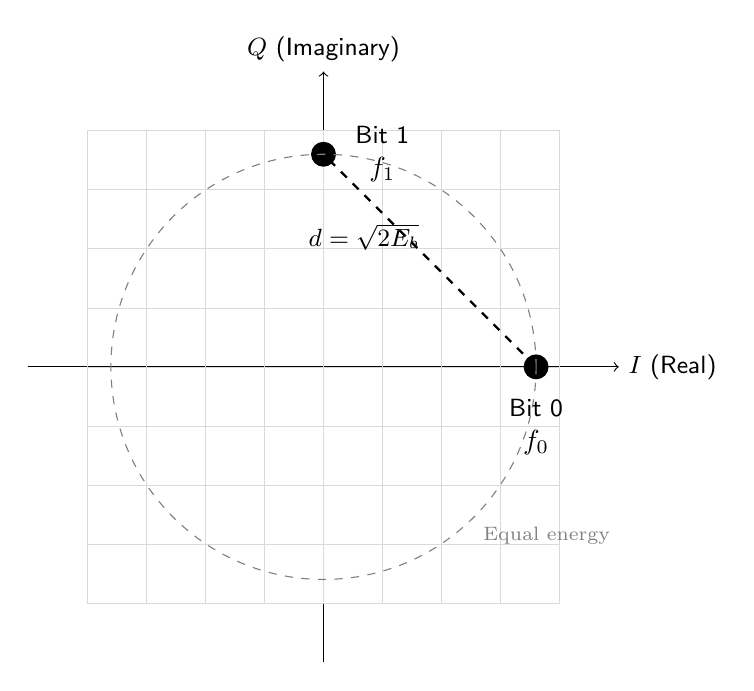
\begin{tikzpicture}[scale=1.5]
% Axes
\draw[->] (-2.5,0) -- (2.5,0) node[right] {\sffamily\small $I$ (Real)};
\draw[->] (0,-2.5) -- (0,2.5) node[above] {\sffamily\small $Q$ (Imaginary)};

% Grid
\draw[very thin,gray!30] (-2,-2) grid[step=0.5] (2,2);

% Constellation points for orthogonal FSK
\fill[black] (1.8,0) circle (3pt);
\fill[black] (0,1.8) circle (3pt);

% Labels
\node[below=8pt,align=center] at (1.8,0) {\sffamily\small Bit 0\\$f_0$};
\node[right=8pt,align=center] at (0,1.8) {\sffamily\small Bit 1\\$f_1$};

% Distance annotation
\draw[<->,thick,dashed] (1.8,0) -- (0,1.8) node[midway,above left] {\sffamily\small $d = \sqrt{2E_b}$};

% Energy circle
\draw[thin,gray,dashed] (0,0) circle (1.8);
\node[below right,gray,font=\scriptsize] at (1.27,-1.27) {Equal energy};
\end{tikzpicture}
\end{center}

For \textbf{orthogonal FSK}, the two signal vectors are perpendicular (90° apart), providing:
\begin{equation}
d = \sqrt{2E_b}
\end{equation}
where $E_b = A^2T_b/2$ is the energy per bit.

\section{Modulation and Demodulation}

\subsection{Transmitter (Modulator)}

The FSK modulator can be implemented using frequency synthesis:

\begin{center}
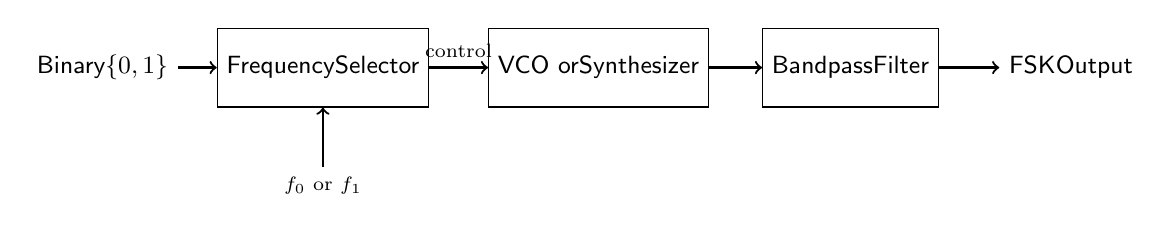
\begin{tikzpicture}[
  block/.style={rectangle, draw, minimum width=2.2cm, minimum height=1cm, font=\sffamily\small},
  node distance=2.2cm,
  font=\small
]
\node (input) {\sffamily Binary\\$\{0, 1\}$};
\node[block, right of=input, node distance=2.8cm] (switch) {Frequency\\Selector};
\node[block, right of=switch, node distance=3.5cm] (vco) {VCO or\\Synthesizer};
\node[block, right of=vco, node distance=3.2cm] (filter) {Bandpass\\Filter};
\node[right of=filter, node distance=2.8cm] (output) {\sffamily FSK\\Output};

\node[below of=switch, node distance=1.5cm, font=\scriptsize, align=center] (freq) {$f_0$ or $f_1$};

\draw[->,thick] (input) -- (switch);
\draw[->,thick] (switch) -- node[above,font=\scriptsize] {control} (vco);
\draw[->,thick] (vco) -- (filter);
\draw[->,thick] (filter) -- (output);
\draw[->,thick] (freq) -- (switch);
\end{tikzpicture}
\end{center}

\textbf{Process:}
\begin{enumerate}
\item \textbf{Data bit determines frequency:} Bit 0 $\rightarrow$ $f_0$, Bit 1 $\rightarrow$ $f_1$
\item \textbf{Voltage-Controlled Oscillator (VCO):} Generates carrier at selected frequency
\item \textbf{Bandpass filter:} Shapes spectrum and removes harmonics
\end{enumerate}

\subsection{Receiver: Non-Coherent Detection}

The most common FSK demodulation uses \textbf{non-coherent detection}, which does not require carrier phase synchronization:

\begin{center}
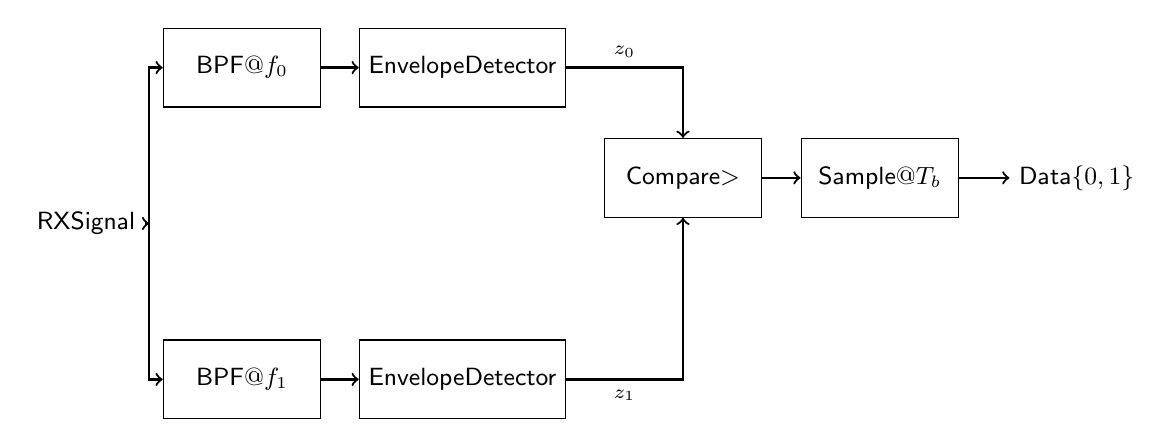
\begin{tikzpicture}[
  block/.style={rectangle, draw, minimum width=2cm, minimum height=1cm, font=\sffamily\small},
  node distance=2cm,
  font=\small
]
\node (input) {\sffamily RX\\Signal};
\node[block, above right of=input, node distance=2.8cm] (bpf0) {BPF\\$@f_0$};
\node[block, right of=bpf0, node distance=2.8cm] (env0) {Envelope\\Detector};
\node[block, below right of=input, node distance=2.8cm] (bpf1) {BPF\\$@f_1$};
\node[block, right of=bpf1, node distance=2.8cm] (env1) {Envelope\\Detector};
\node[block, right of=env0, node distance=2.8cm, yshift=-1.4cm] (comp) {Compare\\$>$};
\node[block, right of=comp, node distance=2.5cm] (sample) {Sample\\$@T_b$};
\node[right of=sample, node distance=2.5cm] (output) {\sffamily Data\\$\{0,1\}$};

\draw[->,thick] (input) -- ++(0.8,0) coordinate (split);
\draw[->,thick] (split) |- (bpf0);
\draw[->,thick] (split) |- (bpf1);
\draw[->,thick] (bpf0) -- (env0);
\draw[->,thick] (bpf1) -- (env1);
\draw[->,thick] (env0) -| node[near start,above,font=\scriptsize] {$z_0$} (comp);
\draw[->,thick] (env1) -| node[near start,below,font=\scriptsize] {$z_1$} (comp);
\draw[->,thick] (comp) -- (sample);
\draw[->,thick] (sample) -- (output);
\end{tikzpicture}
\end{center}

\textbf{Detection process:}
\begin{enumerate}
\item \textbf{Bandpass filters:} Separate $f_0$ and $f_1$ components
\item \textbf{Envelope detectors:} Measure signal amplitude in each channel
\item \textbf{Compare:} Select channel with larger envelope
\item \textbf{Decision:} If $z_0 > z_1$: bit = 0; else: bit = 1
\end{enumerate}

\begin{keyconcept}
\textbf{Non-coherent detection} eliminates the need for carrier phase recovery, significantly simplifying receiver design. The performance penalty is approximately \textbf{1~dB} compared to coherent detection---a worthwhile trade-off for many applications.
\end{keyconcept}

\subsection{Coherent Detection (Optimal)}

For maximum performance, coherent detection uses correlation receivers:

\begin{center}
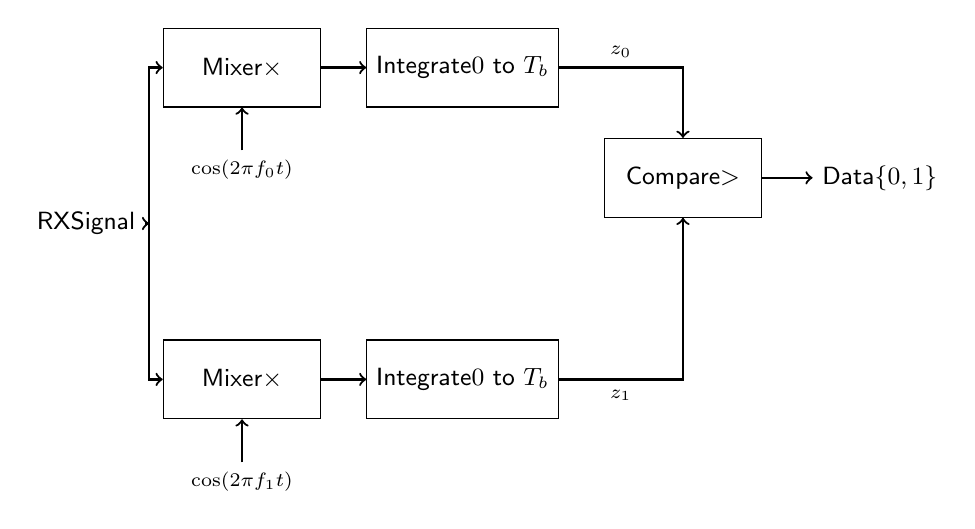
\begin{tikzpicture}[
  block/.style={rectangle, draw, minimum width=2cm, minimum height=1cm, font=\sffamily\small},
  node distance=2cm,
  font=\small
]
\node (input) {\sffamily RX\\Signal};
\node[block, above right of=input, node distance=2.8cm] (mult0) {Mixer\\$\times$};
\node[block, right of=mult0, node distance=2.8cm] (int0) {Integrate\\$0$ to $T_b$};
\node[block, below right of=input, node distance=2.8cm] (mult1) {Mixer\\$\times$};
\node[block, right of=mult1, node distance=2.8cm] (int1) {Integrate\\$0$ to $T_b$};
\node[block, right of=int0, node distance=2.8cm, yshift=-1.4cm] (comp) {Compare\\$>$};
\node[right of=comp, node distance=2.5cm] (output) {\sffamily Data\\$\{0,1\}$};

\node[below of=mult0, node distance=1.3cm, font=\scriptsize, align=center] (lo0) {$\cos(2\pi f_0 t)$};
\node[below of=mult1, node distance=1.3cm, font=\scriptsize, align=center] (lo1) {$\cos(2\pi f_1 t)$};

\draw[->,thick] (input) -- ++(0.8,0) coordinate (split);
\draw[->,thick] (split) |- (mult0);
\draw[->,thick] (split) |- (mult1);
\draw[->,thick] (lo0) -- (mult0);
\draw[->,thick] (lo1) -- (mult1);
\draw[->,thick] (mult0) -- (int0);
\draw[->,thick] (mult1) -- (int1);
\draw[->,thick] (int0) -| node[near start,above,font=\scriptsize] {$z_0$} (comp);
\draw[->,thick] (int1) -| node[near start,below,font=\scriptsize] {$z_1$} (comp);
\draw[->,thick] (comp) -- (output);
\end{tikzpicture}
\end{center}

\textbf{Coherent detection provides optimal performance but requires:}
\begin{itemize}
\item Precise local oscillators at both $f_0$ and $f_1$
\item Phase synchronization (approximately 1~dB improvement over non-coherent)
\item More complex receiver circuitry
\end{itemize}

\begin{warningbox}
\textbf{Frequency accuracy is critical.} The local oscillators must match the transmitter frequencies exactly. Even small frequency offsets degrade performance. For non-coherent FSK, frequency stability requirements are relaxed compared to phase-coherent modulation schemes like BPSK.
\end{warningbox}

\section{Bit Error Rate (BER) Performance}

\subsection{Non-Coherent FSK in AWGN Channel}

For orthogonal non-coherent FSK with envelope detection:
\begin{equation}
\mathrm{BER} = \frac{1}{2}e^{-E_b/(2N_0)}
\end{equation}
where:
\begin{itemize}
\item $E_b = \frac{A^2 T_b}{2}$ = energy per bit (joules)
\item $N_0$ = noise power spectral density (W/Hz)
\end{itemize}

\subsection{Coherent FSK in AWGN Channel}

For orthogonal coherent FSK with correlation detection:
\begin{equation}
\mathrm{BER} = Q\left(\sqrt{\frac{E_b}{N_0}}\right) = \frac{1}{2}\mathrm{erfc}\left(\sqrt{\frac{E_b}{2N_0}}\right)
\end{equation}

\textbf{Performance benchmarks:}

\begin{center}
\begin{tabular}{@{}lrrl@{}}
\toprule
$E_b/N_0$ (dB) & \multicolumn{1}{c}{BER (Non-coh)} & \multicolumn{1}{c}{BER (Coherent)} & Practical Meaning \\
\midrule
5~dB & $6.7 \times 10^{-2}$ & $3.9 \times 10^{-2}$ & 1 error in 15--25 bits \\
10~dB & $6.7 \times 10^{-4}$ & $1.9 \times 10^{-4}$ & 1 error in 1,500--5,000 bits \\
12~dB & $1.2 \times 10^{-4}$ & $2.6 \times 10^{-5}$ & 1 error in 8,000--38,000 bits \\
15~dB & $3.7 \times 10^{-6}$ & $4.3 \times 10^{-7}$ & 1 error in $270$k--$2.3$M bits \\
\bottomrule
\end{tabular}
\end{center}

\textbf{Key insight:} Coherent detection provides approximately \textbf{1~dB} advantage over non-coherent detection at practical BER levels.

\begin{center}\rule{0.5\linewidth}{0.5pt}\end{center}

\subsection{\texorpdfstring{ Advantages \&
Disadvantages}{ Advantages \& Disadvantages}}\label{advantages-disadvantages}

\subsubsection{Advantages}\label{advantages}

\textbf{Constant envelope} - efficient power amplifiers (Class C)
\textbf{Non-coherent detection} - simple receivers \textbf{Robust to
fading} - amplitude variations don\textquotesingle t affect frequency
\textbf{Good for noisy channels} - frequency easier to detect than phase
\textbf{Legacy compatibility} - used in many older systems

\subsubsection{Disadvantages}\label{disadvantages}

\textbf{Poor spectral efficiency} - wider bandwidth than PSK
\textbf{Moderate power efficiency} - 1-2 dB worse than {[}{[}BPSK{]}{]}
\textbf{Frequency stability} - requires accurate oscillators
\textbf{Doppler sensitivity} - frequency shifts problematic

\begin{center}\rule{0.5\linewidth}{0.5pt}\end{center}

\subsection{\texorpdfstring{
Applications}{ Applications}}\label{applications}

\subsubsection{Historical \& Current}\label{historical-current}

\begin{itemize}
\tightlist
\item
  \textbf{Telephone modems} (Bell 103: 1962, 300 baud,
  f\textbackslash textsubscript\{0\}=1070 Hz,
  f\textbackslash textsubscript\{1\}=1270 Hz)
\item
  \textbf{Radio teletype} (RTTY, 1930s-)
\item
  \textbf{Caller ID} (Bell 202: 1200 bps,
  f\textbackslash textsubscript\{0\}=2200 Hz,
  f\textbackslash textsubscript\{1\}=1200 Hz)
\item
  \textbf{Pagers} (POCSAG, FLEX protocols)
\end{itemize}

\subsubsection{Modern}\label{modern}

\begin{itemize}
\tightlist
\item
  \textbf{LoRa} (sub-GHz IoT, chirp spread spectrum FSK)
\item
  \textbf{Bluetooth Low Energy} (GFSK - Gaussian FSK)
\item
  \textbf{Wireless sensor networks} - low power, simple receivers
\item
  \textbf{Optical fiber} (frequency-shifted laser)
\item
  \textbf{{[}{[}AID-Protocol-Case-Study{]}{]}} - 12 kHz FSK sub-carrier
  (11,999/12,001 Hz)
\end{itemize}

\begin{center}\rule{0.5\linewidth}{0.5pt}\end{center}

\subsection{\texorpdfstring{ FSK
Variants}{ FSK Variants}}\label{fsk-variants}

\subsubsection{1. Minimum Shift Keying
(MSK)}\label{minimum-shift-keying-msk}

\textbf{Special case}: h = 0.5 (minimum for orthogonality)

\begin{verbatim}
Properties:
- Continuous phase (no discontinuities)
- Constant envelope
- Bandwidth = 1.5 R_b (narrowest FSK)
- Equivalent to offset QPSK with sinusoidal pulse shaping
\end{verbatim}

\textbf{Used in}: GSM cellular (GMSK - Gaussian MSK)

\begin{center}\rule{0.5\linewidth}{0.5pt}\end{center}

\subsubsection{2. Gaussian FSK (GFSK)}\label{gaussian-fsk-gfsk}

\textbf{MSK + Gaussian pre-modulation filter}

\begin{verbatim}
Purpose: Further reduce spectral sidelobes
Bandwidth: ~1.2-1.5 R_b (depending on BT product)
BT product: Bandwidth × T_b (typical: 0.3-0.5)
\end{verbatim}

\textbf{Used in}: Bluetooth, Zigbee

\begin{center}\rule{0.5\linewidth}{0.5pt}\end{center}

\subsubsection{3. Continuous Phase FSK
(CPFSK)}\label{continuous-phase-fsk-cpfsk}

\textbf{Phase is continuous} across bit boundaries:

\begin{verbatim}
(t) = 2[f_c·t + (hf/2)·^{t} b()d]

Benefits:
- No spectral splatter
- Better spectral efficiency
- Smoother power envelope
\end{verbatim}

\begin{center}\rule{0.5\linewidth}{0.5pt}\end{center}

\subsubsection{4. Multi-Frequency FSK
(MFSK)}\label{multi-frequency-fsk-mfsk}

\textbf{M \textgreater{} 2 frequencies} for higher data rates:

\begin{verbatim}
M symbols  log(M) bits per symbol

Example (4-FSK):
- f: bits 00
- f: bits 01
- f: bits 10
- f: bits 11

Bandwidth: B = M·R_b (wider!)
Power efficiency: Better than BFSK for high M
\end{verbatim}

\textbf{Used in}: HF radio (MT63, Olivia modes)

\begin{center}\rule{0.5\linewidth}{0.5pt}\end{center}

\subsection{\texorpdfstring{ Constellation
Diagram}{ Constellation Diagram}}\label{constellation-diagram}

\textbf{BFSK in frequency space}:

\begin{verbatim}
Frequency
   
f |      Symbol "1"
   |
f_c|       (carrier)
   |
f |      Symbol "0"
   +------------ Time
\end{verbatim}

\textbf{Not a traditional I/Q constellation} (frequency, not
amplitude/phase).

\textbf{Equivalent I/Q representation} (for coherent detection):

\begin{verbatim}
      Q
      
      |
  0  |  1   On real axis, separated
      |
------+------ I
\end{verbatim}

\textbf{Distance between points}: d = \$\textbackslash sqrt\{\}\$(2E\_b)
(for orthogonal FSK)

\begin{center}\rule{0.5\linewidth}{0.5pt}\end{center}

\subsection{\texorpdfstring{ Comparison
Table}{ Comparison Table}}\label{comparison-table}

{\def\LTcaptype{} % do not increment counter
\begin{longtable}[]{@{}
  >{\raggedright\arraybackslash}p{(\linewidth - 10\tabcolsep) * \real{0.1579}}
  >{\raggedright\arraybackslash}p{(\linewidth - 10\tabcolsep) * \real{0.1711}}
  >{\raggedright\arraybackslash}p{(\linewidth - 10\tabcolsep) * \real{0.1447}}
  >{\raggedright\arraybackslash}p{(\linewidth - 10\tabcolsep) * \real{0.2500}}
  >{\raggedright\arraybackslash}p{(\linewidth - 10\tabcolsep) * \real{0.1316}}
  >{\raggedright\arraybackslash}p{(\linewidth - 10\tabcolsep) * \real{0.1447}}@{}}
\toprule\noalign{}
\begin{minipage}[b]{\linewidth}\raggedright
Modulation
\end{minipage} & \begin{minipage}[b]{\linewidth}\raggedright
Bits/Symbol
\end{minipage} & \begin{minipage}[b]{\linewidth}\raggedright
Bandwidth
\end{minipage} & \begin{minipage}[b]{\linewidth}\raggedright
Eb/N0 @ BER 10\^{}-6
\end{minipage} & \begin{minipage}[b]{\linewidth}\raggedright
Envelope
\end{minipage} & \begin{minipage}[b]{\linewidth}\raggedright
Detection
\end{minipage} \\
\midrule\noalign{}
\endhead
\bottomrule\noalign{}
\endlastfoot
{[}{[}On-Off-Keying-(OOK) & OOK{]}{]} & 1 & 2R\_b & 13.5 dB &
Variable \\
\textbf{FSK} & 1 & 2R\_b & 12.5 dB & Constant & Non-coherent \\
\textbf{MSK} & 1 & 1.5R\_b & 10.5 dB & Constant & Coherent \\
{[}{[}BPSK{]}{]} & 1 & R\_b & 10.5 dB & Constant & Coherent \\
{[}{[}QPSK-Modulation & QPSK{]}{]} & 2 & R\_b & 10.5 dB & Constant \\
\end{longtable}
}

\textbf{Key insight}: FSK trades bandwidth for simplicity.
{[}{[}BPSK{]}{]}/{[}{[}QPSK-Modulation\textbar QPSK{]}{]} are more
efficient but require phase synchronization.

\begin{center}\rule{0.5\linewidth}{0.5pt}\end{center}

\subsection{\texorpdfstring{ Key
Takeaways}{ Key Takeaways}}\label{key-takeaways}

\begin{enumerate}
\def\labelenumi{\arabic{enumi}.}
\tightlist
\item
  \textbf{Frequency switching}: Binary data
  \$\textbackslash rightarrow\$ two different frequencies
\item
  \textbf{Constant envelope}: Good for non-linear amplifiers
\item
  \textbf{Non-coherent detection}: Simple receivers, still good
  performance
\item
  \textbf{Bandwidth penalty}: \textasciitilde2\$\textbackslash times\$
  wider than PSK
\item
  \textbf{Robust}: Good for noisy, fading channels
\item
  \textbf{Still widely used}: Bluetooth, LoRa, pagers, caller ID
\item
  \textbf{Gateway to chirp spread spectrum}: LoRa uses frequency chirps
\end{enumerate}

\begin{center}\rule{0.5\linewidth}{0.5pt}\end{center}

\subsection{\texorpdfstring{ See Also}{ See Also}}\label{see-also}

\begin{itemize}
\tightlist
\item
  {[}{[}On-Off-Keying-(OOK){]}{]} - Simpler (amplitude modulation)
\item
  {[}{[}Binary-Phase-Shift-Keying-(BPSK){]}{]} - Alternative (phase
  modulation)
\item
  {[}{[}QPSK-Modulation{]}{]} - More bits per symbol (phase)
\item
  {[}{[}Constellation-Diagrams{]}{]} - Visualizing modulation schemes
\item
  {[}{[}AID-Protocol-Case-Study{]}{]} - Uses 1 bps FSK sub-carrier
  (11,999/12,001 Hz)
\end{itemize}

\begin{center}\rule{0.5\linewidth}{0.5pt}\end{center}

\subsection{\texorpdfstring{ References}{ References}}\label{references}

\begin{enumerate}
\def\labelenumi{\arabic{enumi}.}
\tightlist
\item
  \textbf{Sunde, E.D.} (1946) ``Ideal binary pulse transmission by AM
  and FM'' \emph{Bell Syst. Tech. J.} 25, 1067-1093
\item
  \textbf{de Jager, F. \& Dekker, C.B.} (1978) ``Tamed Frequency
  Modulation'' \emph{IEEE Trans. Comm.} COM-26, 534-542
\item
  \textbf{Proakis, J.G. \& Salehi, M.} (2008) \emph{Digital
  Communications} 5th ed.~(McGraw-Hill)
\item
  \textbf{Sklar, B.} (2001) \emph{Digital Communications} 2nd
  ed.~(Prentice Hall)
\end{enumerate}
